\appendix
\chapter{Test Environment}
\label{App:TestEnv}

This appendix focuses on fully characterizing the hardware and software used in all performance measurements of the application for the different implementations developed.

For the shared memory implementation testing was used three dual-socket multicore systems. The first has two \intel Xeon E5-2650 (Sandy Bridhe architecture) \ref{Intel:E52650}, using the Quick Path Interconnect (QPI) interface between CPUs, in a Non Unified Memory Access model (NUMA), meaning that the latency of a CPU acessing its own memory bank is lower than accessing the other CPU memory bank. The QPI interface can perform up to 8 GT/s (giga transfers per second) of 2 bytes packets, in each of the two unidirectional links, with a total bandwidth of 32 GB/s. Figure \ref{fig:SystemModel} illustrates the architectural model of this system. The system features 64 GB of DDR3 RAM with a speed of 1333 MHz, for a maximum bandwidth of ZZ GB/s, measured with the STREAM benchmark \ref{STREAM}.

\begin{figure}[!htp]
	\begin{center}
		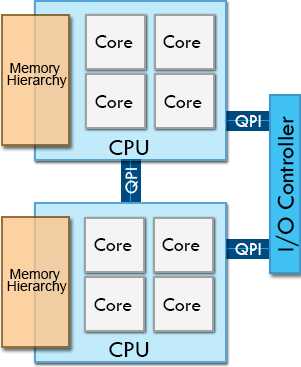
\includegraphics[scale=0.5]{../../common/img/numa_qpi.png}
		\caption{Schematic representation of a NUMA system with QPI interface.}
		\label{fig:SystemModel}
	\end{center}
\end{figure}

The second system has the same amount of RAM at the same speed, with a maximum bandwidth of ZZ GB/s. The two CPUs are \intel Xeon X5650 (Nehalem architecture). The difference of memory bandwidth is due to the different memory controllers, while the one in Nehalem has 3 memory channels the one in Sandy Bridge has 4. The two CPUs are interconnect by a QPI interface, but with a different speed than the Sandy Bridge, performing 6 GT/s in each of the two unidirectional channels, for a total bandwidth of 24 GB/s.

The third system features two \amd Opteron 6174, being the system with more physical cores. It has 64 GB of DDR3 RAM at 1333 MHz, with a maximum measured bandwidth of ZZ GB/s. \amd uses HyperTransport (HT) 3.0 technology, a point-to-point interconnection similar to QPI capable of transmitting 4 byte packets through two links, for an aggregate bandwidth of 51.2 GB/s. The characteristics of the CPUs on the three systems are presented in table \ref{tab:CPUS}.

\begin{table}[!htp]
	\begin{center}
		\begin{tabular}{|c|c|c|c|}
			\hline
			\textbf{CPU} & \intel Xeon E5-2650 & \intel Xeon X5650 & \amd Opteron 6174 \\ \hline
			\textbf{Architecture} & Sandy Bridge & Nehalem & Magny\-Cours \\ \hline
			\textbf{Clock Freq.} & 2.0 GHz & 2.66 GHz & 2.2 GHz \\ \hline
			\textbf{\# of Cores} & 8 & 6 & 12 \\ \hline
			\textbf{\# of Threads} & 16 & 12 & 12 \\ \hline
			\textbf{L1 Cache} & \specialcell{32 KB I. +\\32 KB D. per Core} & \specialcell{32 KB I. +\\32 KB D. per Core} & \specialcell{64 KB I. +\\64 KB D. per Core} \\ \hline
			\textbf{L2 Cache} & 256 KB per Core & 256 KB per Core & 512 KB per Core \\ \hline
			\textbf{L3 Cache} & 20 MB shared & 12 MB shared & \- \\ \hline
			\textbf{CPU Interconnection} & QPI @4.0 GHz & QPI @3.2 GHz & HT @3.2 GHz \\ \hline
			\textbf{ISE} & AVX & SSE 4.2 & SSE 4a \\
			\hline
		\end{tabular}
		\caption{Characterization of the CPUs featured in the three test systems.}
		\label{tab:CPUS}
	\end{center}
\end{table}

The Roofline model \ref{Roofline} was used characterize the system in terms of attainable peak performance. This model uses two metrics for the performance calculation: the peak CPU performance and the memory bandwidth. With the peak values of these two metrics a roofline is drawn, being the theoretical limit for the performance on the system. Then, other ceilings can be added, which further limit the maximum attainable performance. The classic Roofline uses float point computation as the peak CPU performance metric. It may be a good metric for heavy computational algorithms, such as matrix multiplication, but the type operations on the critical region (\ttDilepKinFit function) are much more varied, as shown in the instruction mix presented in section \ref{ttDilep}. Instead, the computational intensity was used for measuring the CPU peak performance, as it considers all types of instructions.

Figure \ref{fig:Roofline} illustrates the Roofline model for the three systems.

\todo{Rooflines...}

The compiler used was the GNU compiler version 4.8, using the -O3 optimizations and the AVX/SSE 4.2/SSE 4a (depending on the CPU architecture) instruction set on the code regions that the compiler sees fit. The compiler features the OpenMP version 3.2 used in the shared memory implementation. For the GPU implementation was used the CUDA 5 SDK, in conjunction with the GNU compiler version 4.6.3 for the code to run on the CPU (any later versions are not supported by the \nvidia NVCC compiler). The ROOT \ref{CERN:ROOT} version used was the 5.34/05. All libraries/frameworks used were compiled with compliance to the C++ 11 specifications to ensure, among other things, thread safety on memory allocations. Was used the Performance API version 5.0 for measuring the hardware counters of the different CPUs for the characterization of \ttDilepKinFit.
